\subsection{Code Generator}

In this section you will learn how to implement the code generator for 
the target application. For simplicity, the code generator templates are placed
in the \texttt{org.eclipse.xtext.example.ql} project in a sub-package \texttt{generator}. 
Usually it would be better to create a separate project which contains the generator,
since the language is independent from a single target platform. It would
be possible to create different code generators for different target platforms,
and it would be better to implement each of them as separate projects.

Generator templates in Xtend are implementations of the \texttt{IGenerator}
interface:

\begin{lstlisting}[language=Java]
package org.eclipse.xtext.generator;

public interface IGenerator {
	/**
	 * @param input - the input for which to generate resources
	 * @param fsa - file system access to be used to generate files
	 */
	public void doGenerate(Resource input, IFileSystemAccess fsa);
}
\end{lstlisting}

\subsubsection {Dispatcher template}
\label{sec:dispatcherTemplate}

The code generator is invoked with a \texttt{Resource} instance, which holds a \texttt{Questionnaire}
instance. We have to generate multiple artifacts for each resource, so it is a common 
pattern to create a template class which serves as entry point and dispatches to other
template classes to create the artifacts. Usually one template per artifact is
created.

Create the class \texttt{Root.java} in 
package \texttt{org.eclipse.xtext.example.ql.generator}:

\begin{lstlisting}[language=Java]
package org.eclipse.xtext.example.ql.generator;

import javax.inject.Inject;

import org.eclipse.emf.ecore.resource.Resource;
import org.eclipse.xtext.generator.IFileSystemAccess;
import org.eclipse.xtext.generator.IGenerator;
import org.eclipse.xtext.xbase.compiler.JvmModelGenerator;

@SuppressWarnings("restriction")
public class Root implements IGenerator {
  @Inject
  JvmModelGenerator jvmModelGenerator;

  public void doGenerate(Resource input, IFileSystemAccess fsa) {
    // dispatch to other generators
    jvmModelGenerator.doGenerate(input, fsa);
  }
}
\end{lstlisting}

As a first generator to which is dispatched, we inject an instance of
\texttt{JvmModelGenerator}. This is a standard generator shipped with Xtext which
translates types inferred by the Jvm Model Inferrer to Java classes.
In our case, the Java class for Forms are generated by the
\texttt{JvmModelGenerator}. In JSF terms, we speek of the \emph{Backing Bean}.
 
Next, Xtext has to know that \texttt{Root} is the template that has to be invoked
as generator implementation. Whenever a default implementation must be exchanged
by a custom one, this has to be added or overridden in the respective Guice
module.
In the case of the custom \texttt{IGenerator} implementation, this has to be added to the
\texttt{QlDslRuntimeModule} class. Open this class and add a configuration that
binds the \texttt{IGenerator} interface to the \texttt{Root} class.

\begin{lstlisting}[language=Java]
  @Override
  public Class<? extends IGenerator> bindIGenerator() {
    return Root.class;
  }
\end{lstlisting}

Now we are ready to add additional templates and register them in the
\texttt{Root} class.
\subsubsection{Output Configuration Provider}
\label{sec:outputConfigurationProvider}

In JSF applications all the web related content is normally placed under
\texttt{./WebContent} instead of \texttt{./src-gen}, which is mostly used as
output for generated java artifacts. We want to adapt to the web applications
structure and seperate generated java classes and JSF artifacts from each other. For that purposes add
a class called \texttt{JsfOutputConfigurationProvider.java} derived from
\texttt{org.eclipse.xtext.generator.OutputConfigurationProvider} 
\footnote{\url{http://xtextcasts.org/episodes/15-output-configurations}} within package
\texttt{org.eclipse.xtext.example.ql.generator}.The new provider adds an
additional \newline \texttt{OutputConfiguration} for the ouput directory
\texttt{./WebContent} as shown in the listing below.

\begin{lstlisting}[language=Java]
package org.eclipse.xtext.example.ql.generator;

import java.util.Set;

import org.eclipse.xtext.generator.OutputConfiguration;
import org.eclipse.xtext.generator.OutputConfigurationProvider;

public class JSFOutputConfigurationProvider extends OutputConfigurationProvider {

  public final String WEB_CONTENT = "WebContent";

  /**
   * @return a set of {@link OutputConfiguration} available for the generator
   */
  public Set<OutputConfiguration> getOutputConfigurations() {
    Set<OutputConfiguration> outputConfigurations = super
        .getOutputConfigurations();

    OutputConfiguration webContent = new OutputConfiguration(WEB_CONTENT);
    webContent
        .setDescription("Read-only Output Folder for web generated application artifacts");
    webContent.setOutputDirectory("./WebContent");
    webContent.setOverrideExistingResources(true);
    webContent.setCreateOutputDirectory(true);
    webContent.setCleanUpDerivedResources(true);
    webContent.setSetDerivedProperty(true);
    outputConfigurations.add(webContent);

    return outputConfigurations;
  }
}
\end{lstlisting}

The interface \texttt{OutputConfiguration} provides several options to configure
the behavior of the so called \texttt{Outlet}. We use the defaults as in
\texttt{OutputConfigurationProvider} except its name, description and outputDirectoy.

Our \texttt{JsfOutputConfigurationProvider} can be bound in the
\texttt{QlDslRuntimeModule} by overriding/extending the method
\texttt{configure}.

\begin{lstlisting}[language=Java]
@Override public void configure(Binder binder) {
    super.configure(binder);
    binder.bind(IOutputConfigurationProvider.class)
        .to(JSFOutputConfigurationProvider.class).in(Singleton.class);
  }
 \end{lstlisting}
 
After this step we can refer to the additional \texttt{OutputConfiguration} in
generators by use of the constant \texttt{WEB\_CONTENT} defined in class
\texttt{JsfOutputConfigurationProvider}.

\subsubsection {JSF Generator}
\label{sec:jsfGenerator}
 
 After creation of the class \texttt{Root} in section
\ref{sec:dispatcherTemplate} where we easily can
add new Generators and the defintion of the
\texttt{JsfOutputConfigurationProvider} in section \ref{sec:outputConfigurationProvider}
which prvides an output folder for JSF
artifacts, we use the \emph{New Xtend Class Wizard} to create a new Xtend class
called \texttt{JSFGenerator.xtend} in package \texttt{org.eclipse.xtext.example.ql.generator}.

This class will be our entry point to generate JSF related artifacts. The
\emph{New Xtend Class Wizard} provides the possibility to bind interfaces to the
new class by use of the \texttt{Add} button near the interface section.

\begin{center}
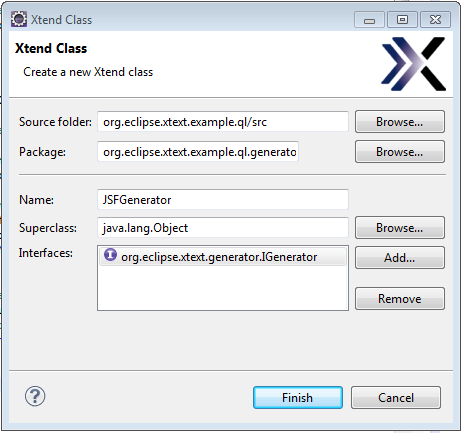
\includegraphics[width=8cm]{./images/chapter02/newXtendClassWizard.png}
\end{center}

As we want to create a new generator we add the interface
\texttt{org.eclipse.xtext.generator.IGenerator} to our new Xtend class.
After typing in the package, the name and the interface of our new Xtend class
as shown in the figure above, we can finish the
wizard so that the class shown in the following listing
will be created in our project.

\begin{lstlisting}[language=Xtend] 
package org.eclipse.xtext.example.ql.generator

import org.eclipse.xtext.generator.IGenerator
import org.eclipse.emf.ecore.resource.Resource
import org.eclipse.xtext.generator.IFileSystemAccess

class JSFGenerator implements IGenerator {
	
	override doGenerate(Resource input, IFileSystemAccess fsa) {
		throw new UnsupportedOperationException("TODO: auto-generated method stub")
	}
}
\end{lstlisting}

To get the created \texttt{JSFGenarator} executed we have to inject and dispatch
to it in our dispatcher template \texttt{Root.java} which was created in section
\ref{sec:dispatcherTemplate} earlier.

\begin{lstlisting}[language=Java] 
 package org.eclipse.xtext.example.ql.generator;

import javax.inject.Inject;

import org.eclipse.emf.ecore.resource.Resource;
import org.eclipse.xtext.generator.IFileSystemAccess;
import org.eclipse.xtext.generator.IGenerator;
import org.eclipse.xtext.xbase.compiler.JvmModelGenerator;

public class Root implements IGenerator {
  @Inject
  JvmModelGenerator jvmModelGenerator;
  @Inject
  JSFGenerator jsfGenerator;

  public void doGenerate(Resource input, IFileSystemAccess fsa) {
    // dispatch to other generators
    jvmModelGenerator.doGenerate(input, fsa);
    jsfGenerator.doGenerate(input, fsa);
  } 
}
\end{lstlisting}

Now it is time to add some functionality to the \texttt{JSFGenarator}. Open the
file \texttt{JSFGenarator.xtend} and go to the \texttt{doGenerate} extension
which is responsible to generate artifacts. Delete the auto-generated body of
the extension - initially it just throws an
\texttt{UnsupportedOperationException} - and add the following lines as first
statements to prevent execution of the generator if the file extension does not fit.

\begin{lstlisting}[language=Java] 
  if (input.URI.fileExtension!="ql")
            return
\end{lstlisting}

After this pre condition is passed we want to execute the generator logic for
our model so it is a good idea to save the models root node in a variable.

\begin{lstlisting}[language=Java] 
  val questionnaire = input.contents.head as Questionnaire 
\end{lstlisting}

Because we want to generate JSF artifacts into the \texttt{WebContent} folder
in the following steps we let Guice add a \texttt{JSFOutputConfigurationProvider}
extension to our \texttt{JSFGenerator}.

\begin{lstlisting}[language=Java] 
class JSFGenerator implements IGenerator{
  @Inject extension JSFOutputConfigurationProvider
  ...
 }
\end{lstlisting}

After this we have the possibility to use the \texttt{WEB\_CONTENT} outlet
constant as described in section \ref{sec:outputConfigurationProvider}.\newline

The following section \ref{sec:jsfGenerator} will describe the different
extensions of the JSFGenerator which are responsible to generate the JSF artifacts described in
\ref{subsec:referenceImpl}. In a real world project it can be a good decision to
seperate different artifacts in different \texttt{Xtend} files. Our sample is a
very simple one, so we will add a new extension definition derived from the
sample below to the \texttt{JSFGenerator.xtend} class which encapsulates the
logic to generate a single artifact.

\begin{lstlisting}[language=HTML] 
  def generate_Artifact (EObject modelInfo)
  '''<?xml version='1.0' encoding='UTF-8' ?>
      <!-- @generated -->
      <!DOCTYPE html PUBLIC "-//W3C//DTD XHTML 1.0 Transitional//EN" "http://www.w3.org/TR/xhtml1/DTD/xhtml1-transitional.dtd">
      <html xmlns="http://www.w3.org/1999/xhtml"
        xmlns:h="http://java.sun.com/jsf/html"
        xmlns:ui="http://java.sun.com/jsf/facelets">
     	... artifact content
      </html>
  '''
\end{lstlisting}

To get a valid xhtml page we have to generate the DOCTYPE
and HTML tag into each XHTML file. It was replaced in the 
listings of the following sections to focus on what matters.
 To get simple access to all generated forms in the application
 we want to generate an index page where a link is included for each form which is defined
in our model.
The generated index page should be saved in a file called index.xhtml within a
subfolder \texttt{'generated/forms/'} of the \texttt{WEB\_CONTENT}
OutputConfiguration created in section \ref{sec:outputConfigurationProvider}.

\begin{lstlisting}[language=Java] 
class JSFGenerator implements IGenerator{
  @Inject extension JSFOutputConfigurationProvider
  @Inject extension QlDslExtensions
  
  override doGenerate(Resource input, IFileSystemAccess fsa) {
        if (input.URI.fileExtension!="ql")
            return
		// model root
        val questionnaire = input.contents.head as Questionnaire
		// generate index page with links to generated forms
        val contentIndex  = generate_FormIndex(questionnaire.forms)
        val fileNameIndex = "generated/forms/index.xhtml"
        fsa.generateFile(fileNameIndex,WEB_CONTENT, contentIndex)
        ...
  }
  ...
 }
      
\end{lstlisting}

For the new artifact add a new extension called \texttt{def
generate\_FormIndex}.
It receives a list of \texttt{Form} elements. In a short loop it generates an
\texttt{html:outputlink} for each form of the given model. Because
\texttt{doGenerate} is called for each QL resource the generator currently has the limitation that all
QL model elements have to be defined within the same QL resource to ensure
generation of a correct form index page.

\begin{lstlisting}[language=Xtend] 
  def generate_FormIndex (List<Form> forms)
  '''...
      <ui:composition template="/index.xhtml">
        <ui:define name="content">
        
        «FOR elem: forms SEPARATOR "<br/>"»
          <h:outputLink value="«elem.name».jsf">«elem.name»</h:outputLink>
        «ENDFOR»
        
        </ui:define>
      </ui:composition>
      ... 
  '''
\end{lstlisting}
 
By using the attribute \texttt{template} of a \texttt{composition} tag as
already described in \ref{subsec:referenceMainLayout}, the structure and styles of
index.xhtml will be derived in our form index page. Our generated form index
needs a \texttt{index.xhtml} in the applications root folder which itself or one of its
parent templates defines a \texttt{facelet:insert} section with name 'content'
like described in section \ref{subsec:referenceMainLayout}.

To get the possibility to change the template for all generated files in
a single file easily later we will use the generated form index as template for
generated form pages in a later step. The generated form index looks similar to
the one described in section \ref{subsec:referenceForms}.

 \ldots  TODO
\subparagraph{JSF Form base}

\subparagraph{JSF Form composite}

 \ldots  be continued